\section{przypadek testowy 4}
\subsection{Cel: }
Celem badania jest sprawdzenie czy rzeczywista złożoność czasowa dla algorytmu two-opt jest zgodna z oczekiwanym \(O(n^3)\).
\subsection{Założenia: }
Podczas badania korzystać będziemy z losowych instancji grafów pełnych, symetrycznych o \(n \in \{ 30, 40, 50 \ldots 100 \}\) wierzchołkach. Badanie czasu każdego rozmiaru grafów zostało powtórzone 30 razy.

\subsection{Wyniki: }
Tabela czasów przedstawia czasy wykonania programu. Dane w tabach, dla czytelności, zostały zaokrąglone do 3 miejsc po przecinku. W dalszych obliczeniach korzystaliśmy z danych dokładnych zamieszczonych w pliku csv/xlsx.
\begin{table}[H]
  \centering
  \begin{tabular}{|c|c|c|c|c|c|c|c|}
  \hline
      30 & 40 & 50 & 60 & 70 & 80 & 90 & 100 \\ \hline \hline
      0.479 & 0.645 & 0.889 & 1.399 & 2.497 & 4.054 & 6.243 & 8.768 \\ \hline
      0.477 & 0.629 & 0.889 & 1.397 & 2.494 & 3.746 & 6.227 & 8.748 \\ \hline
      0.478 & 0.662 & 0.884 & 1.400 & 2.473 & 3.726 & 6.265 & 8.781 \\ \hline
      0.473 & 0.641 & 0.881 & 1.388 & 2.506 & 3.768 & 6.229 & 8.796 \\ \hline
      0.472 & 0.645 & 0.889 & 1.398 & 2.457 & 3.697 & 6.254 & 8.921 \\ \hline
      0.480 & 0.641 & 0.885 & 1.397 & 2.469 & 3.713 & 6.253 & 8.829 \\ \hline
      0.474 & 0.637 & 0.885 & 1.400 & 2.457 & 3.688 & 6.238 & 8.791 \\ \hline
      0.477 & 0.640 & 0.886 & 1.406 & 2.467 & 3.724 & 6.211 & 8.824 \\ \hline
      0.479 & 0.647 & 0.882 & 1.545 & 2.629 & 3.687 & 6.264 & 8.759 \\ \hline
      0.471 & 0.637 & 0.884 & 1.508 & 2.504 & 3.666 & 6.294 & 8.732 \\ \hline
      0.490 & 0.639 & 0.889 & 1.466 & 2.608 & 3.738 & 6.386 & 8.696 \\ \hline
      0.479 & 0.639 & 0.882 & 1.473 & 2.458 & 3.763 & 6.405 & 8.770 \\ \hline
      0.481 & 0.642 & 0.892 & 1.477 & 2.464 & 3.816 & 6.356 & 8.747 \\ \hline
      0.476 & 0.639 & 0.884 & 1.460 & 2.461 & 3.720 & 6.398 & 8.875 \\ \hline
      0.480 & 0.642 & 0.883 & 1.459 & 2.465 & 3.743 & 6.442 & 8.904 \\ \hline
      0.476 & 0.640 & 0.903 & 1.471 & 2.514 & 3.714 & 6.347 & 8.988 \\ \hline
      0.477 & 0.644 & 0.878 & 1.472 & 2.458 & 3.762 & 6.451 & 8.958 \\ \hline
      0.464 & 0.639 & 0.889 & 1.468 & 2.485 & 3.759 & 6.272 & 8.829 \\ \hline
      0.496 & 0.637 & 0.886 & 1.539 & 2.445 & 3.754 & 6.491 & 8.984 \\ \hline
      0.477 & 0.642 & 0.880 & 1.478 & 2.452 & 3.720 & 6.261 & 8.798 \\ \hline
      0.474 & 0.639 & 0.882 & 1.469 & 2.458 & 3.729 & 6.367 & 8.872 \\ \hline
      0.476 & 0.644 & 0.884 & 1.472 & 2.458 & 3.784 & 6.423 & 8.805 \\ \hline
      0.611 & 0.641 & 0.884 & 1.462 & 2.438 & 3.804 & 6.218 & 8.701 \\ \hline
      0.472 & 0.638 & 0.883 & 1.447 & 2.449 & 3.679 & 6.197 & 8.705 \\ \hline
      0.480 & 0.645 & 0.895 & 1.454 & 2.856 & 3.617 & 6.245 & 8.872 \\ \hline
      0.472 & 0.641 & 0.897 & 1.461 & 2.449 & 3.697 & 6.195 & 8.894 \\ \hline
      0.473 & 0.641 & 0.873 & 1.485 & 2.453 & 3.659 & 6.261 & 8.802 \\ \hline
      0.485 & 0.639 & 0.898 & 1.474 & 2.435 & 3.657 & 6.280 & 8.900 \\ \hline
      0.478 & 0.642 & 0.880 & 1.515 & 2.462 & 3.670 & 6.302 & 8.923 \\ \hline
      0.471 & 0.642 & 0.888 & 1.600 & 2.455 & 3.761 & 6.310 & 8.987 \\ \hline
  \end{tabular}
  \caption{tabela czasów dla poszczególnych n, czasy podane w sekundach}
\end{table}

\begin{table}[H]
  \centering
  \begin{tabular}{|c||c|c|c|c|c|c|c|c| }
  \hline
  n & 30 & 40 & 50 & 60 & 70 & 80 & 90 \\ \hline \hline
  T & 0.482 & 0.641 & 0.886 & 1.461 & 2.489 & 3.734 & 6.303 \\ \hline
  SD & 0.025 & 0.005 & 0.006 & 0.050 & 0.082 & 0.076 & 0.083 \\ \hline
  SE & 0.005 & 0.001 & 0.001 & 0.009 & 0.015 & 0.014 & 0.015 \\ \hline
  \end{tabular}
  \caption{T - średni czas wykoniania (w sekundach), SD - odchylenie standardowe, SE - błąd standardowy}
\end{table}

Odchylenie standardowe oraz błąd standardowy zostały obliczone według wzorów: \\
Odchylenie standardowe:
\[ \sigma = \sqrt{\frac{\sum_{n = 1}^{100}(\bar{x} - x_n)^2}{100}} \]
Błąd standardowe:
\[ \sigma_{\bar{x}} = \frac{\sigma}{\sqrt{100}} \]

\subsection{Wykresy: }
\begin{figure}[htb]
    \centering
    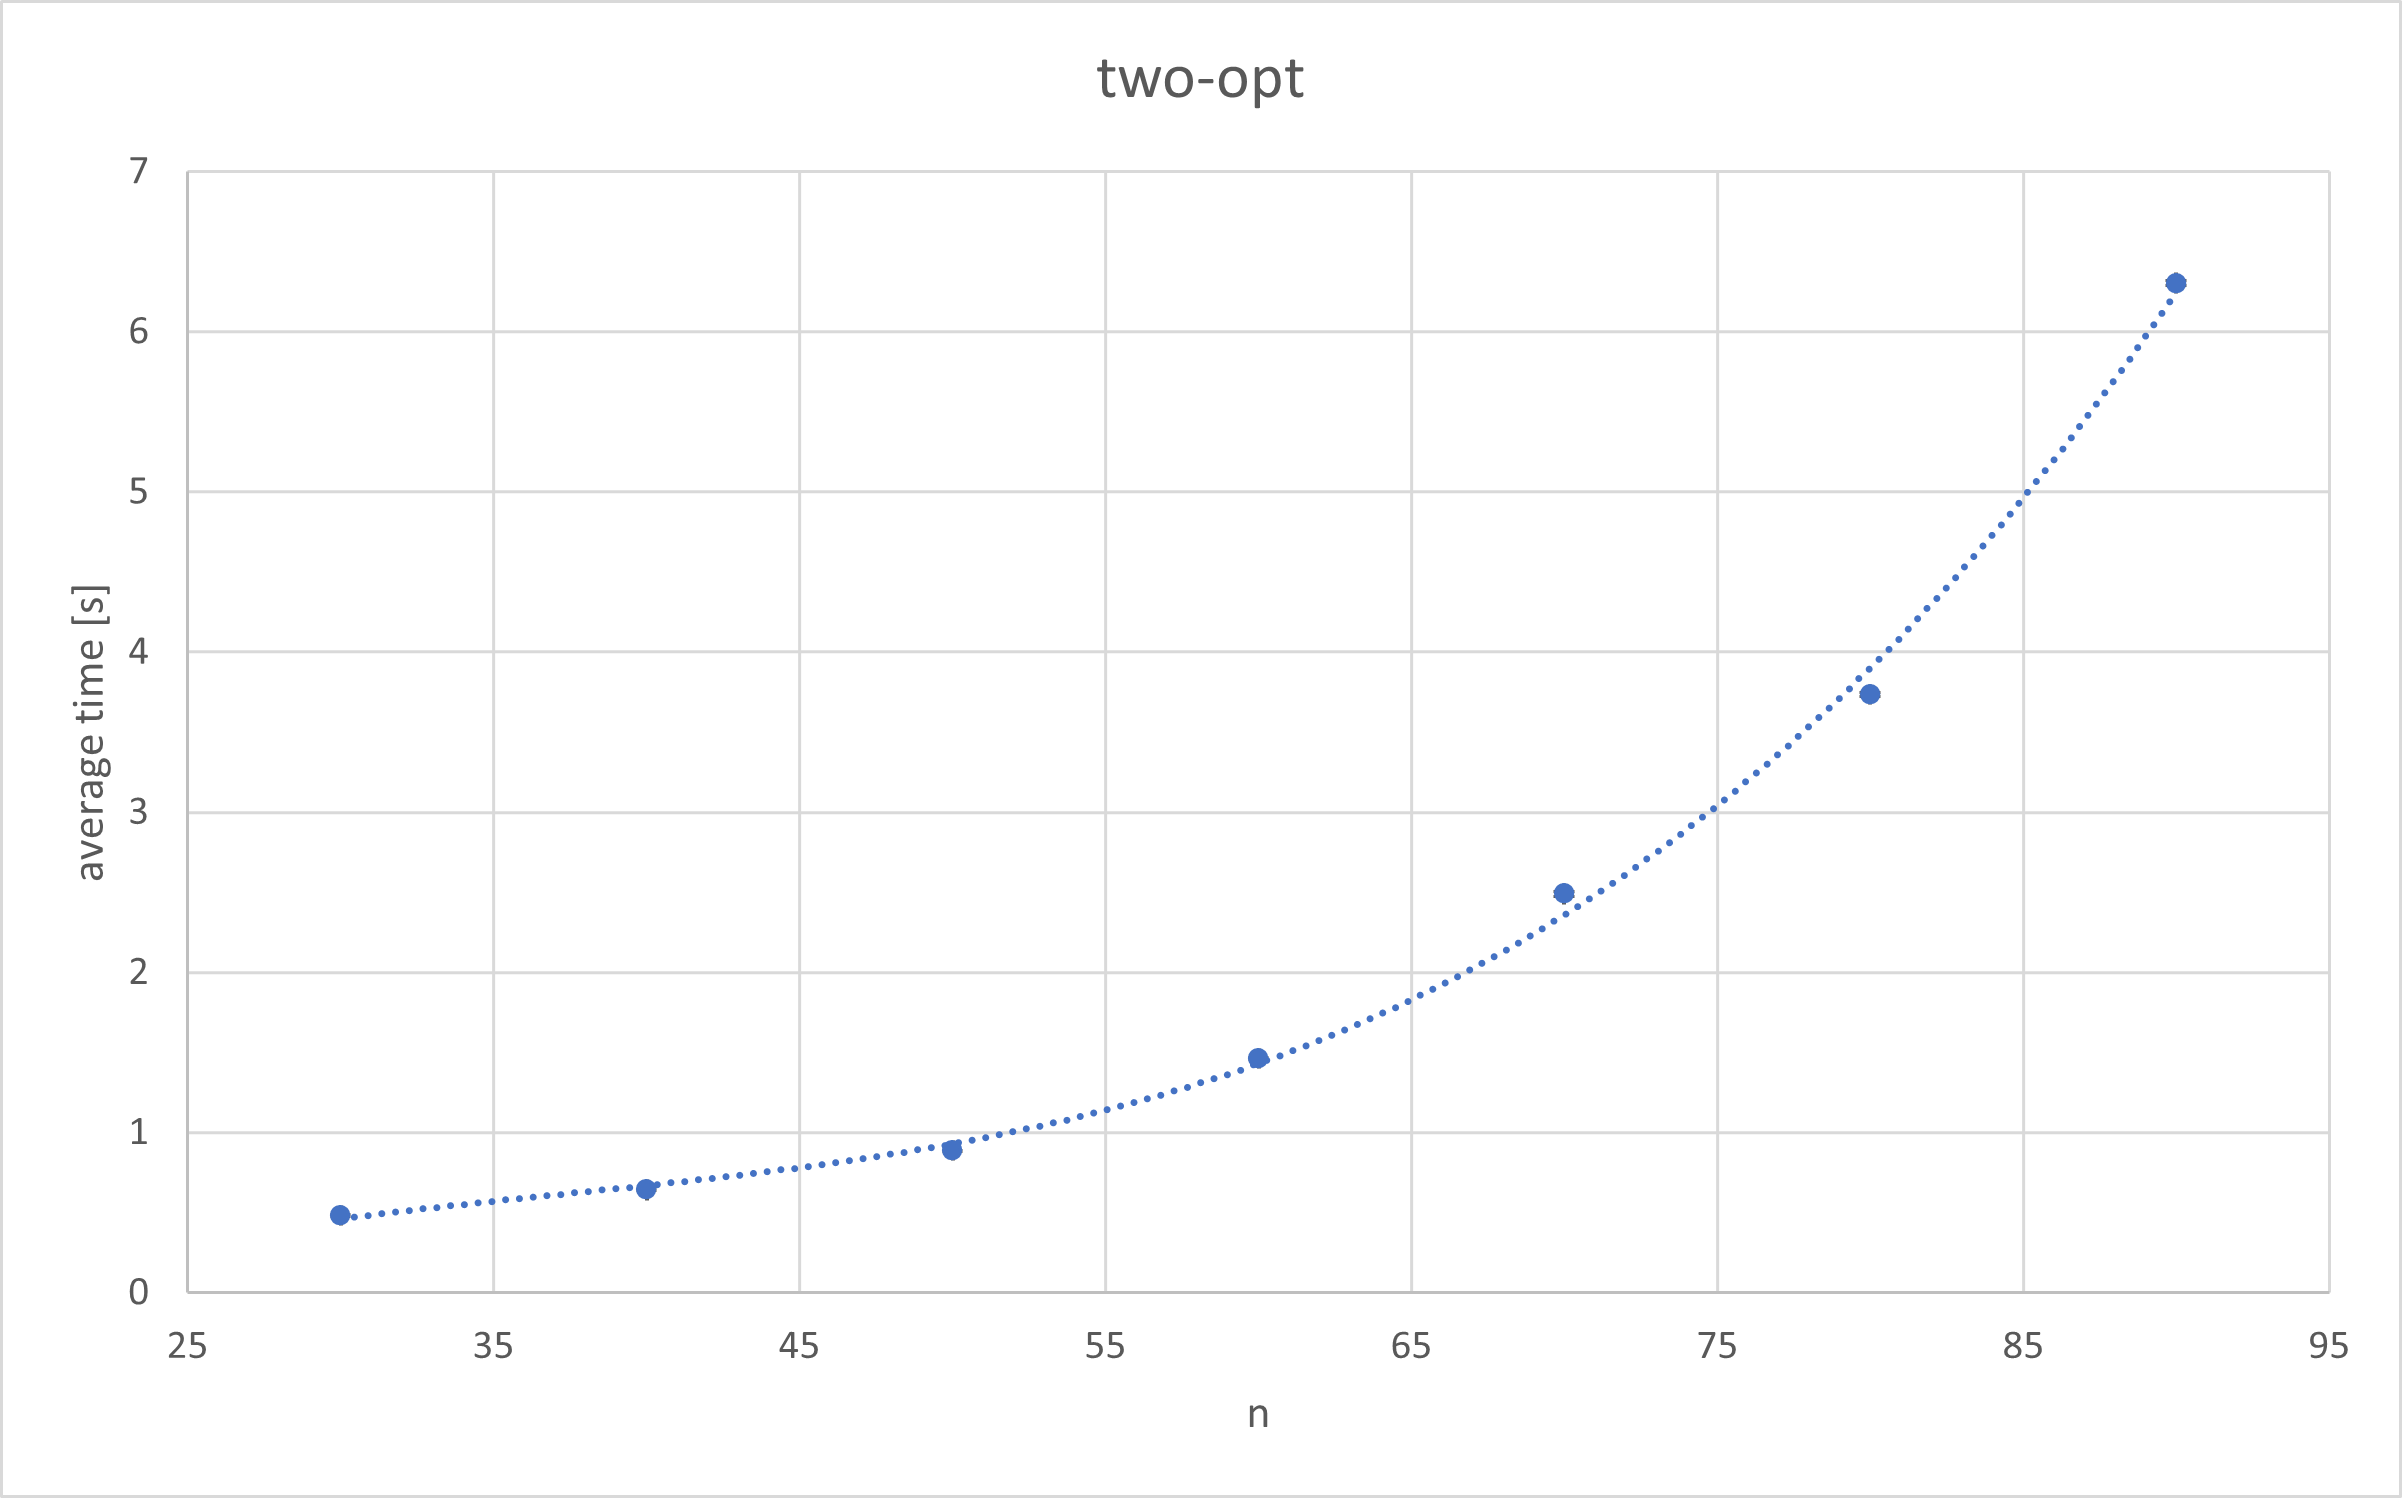
\includegraphics[width=\linewidth]{chart_test3.png}
    \caption{średnie czasy wykonania wraz z błędami standardowymi}
\end{figure}
Na osi OX wykresu naniesione zostały \(n\) dla których wykonywany był pomniar, na osi OY uśrednione wartości czasów wykonania wraz z zaznaczonymi błędami standardowymi.

\subsection{Wnioski: }
Zmierzone dane potwierdziły tezę, że złożoność czasowa metody two-opt ustalonym jest \(O(n^3)\). 

